% ===============================================================================
\section{Overview}
The \wingjMatlab provides a Matlab environment for generating statistics and plots from structure and expression datasets exported from \wingj. The toolbox contains four packages:

\begin{itemize}
 \item \textbf{Structure measurements}. Takes structure measurements from many experiments as input and generates statistics and boxplots. For instance, this package can be used to compare the area of each of the four compartments DA, DP, VA, and VA included in the \droso wing pouch or embryo for wild type and mutant experiments.
 \item \textbf{Expression profiles}. Takes expression profiles from many experiments as input and integrates them to generate \textit{mean expression profiles}. An example is given in \figureref{fig:wingj_expression_profiles_demo}.
 \item \textbf{Expression maps}. Takes individual circular expression maps from many experiments as input to compute mean and standard deviation expression maps. An example is given in \figureref{fig:wingj_expression_maps_circular_demo}.
 \item \textbf{Cell nuclei detection}. Provides a 3D cell nuclei detection method based on a watershed transform to reconstruct 3D nuclei from a stack of confocal fluorescence images. A nuclear staining such as TO-PRO \autocite{suzuki1997dna} or histone GFP constructs \autocite{kanda1998histone} is required.
\end{itemize}

The \wingjMatlab package relies on the file naming convention and directory structure introduced in \sectionref{chap:convention}. In addition, the filenames of the structure and expression datasets must respect the formats introduced in their respective section. For a concrete example of file naming and directory organization, please have a look at the folder \emph{benchmarks} included in the \wingjMatlab. Here, the folder \emph{benchmarks} is an \emph{experiments repository} (\sectionref{sec:experiment_repository}) and contains data from several wings quantified using \wingj. This folder also provides the required input data for running the example \matlab scripts described in the subsequent sections.

% ===============================================================================
\section{Structure measurements}\label{sec:matlab_structure}
Structure datasets described in \sectionref{sec:wingj_structure_dataset} include an XML file that contains the measurements taken from a structure model previously inferred in \sectionref{chap:structure}. Each measurement (e.g. length of the A/P and D/V compartment boundaries, area/perimeter of the wing or embryo, etc.) is identified by a different \emph{\wingj code}. This code is then given to the \matlab scripts to select the measurement data to consider in plot and in statistical analyses.

\begin{itemize}
 \item \textbf{Length of the A/P and D/V compartment boundaries} (\textit{AP.length}, \textit{DV.length})
 \item \textbf{Length of the four \textit{half-boundaries} C-V, C-D, C-A, and C-P} that are part of the A/P and D/V compartment boundaries where C is the intersection of the A/P and D/V boundaries and D, V, A, and P correspond to the points where the A/P and D/V boundaries meet the outer border (or contour) of the structure model (\textit{CV.length}, \textit{CD.length}, etc.)
 \item \textbf{Perimeter and area of the four compartments DA, DP, VA, and VP} that form the structure model (\textit{da.perimeter}, \textit{da.area}, \textit{dp.perimeter}, \textit{dp.area}, etc.)
 \item \textbf{Perimeter and area of the structure model} (\textit{structure.perimeter} and \textit{structure.area})
\end{itemize}

First, find the example script \textit{benchmark\_structure.m} and run it. The output obtained should match the one given in \figureref{fig:matlab_structure}. The script contains many detailed comments that explain step by step what is performed (comments start with the character '\%'). Here, we only provide a broad overview of tools available in the \wingjMatlab.\\

\begin{figure}[!h]
\centering
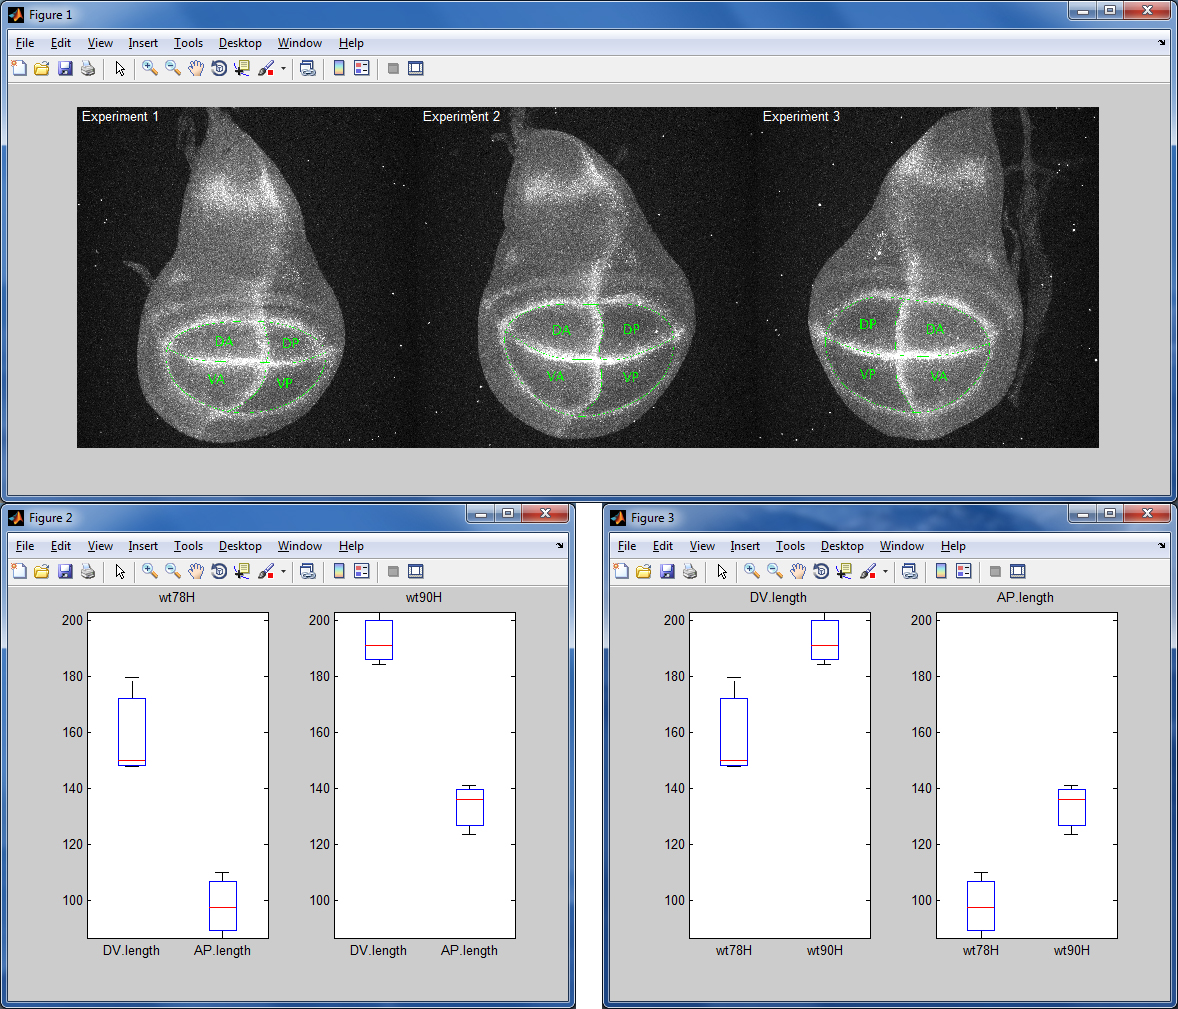
\includegraphics[scale=0.35]{images/matlab_structure.jpg}
\caption{\textbf{Output of the \wingj \matlab script \textit{benchmark\_structure.m}.} For each experiment selected, the first window shows a preview of the structure model inferred by \wingj (requires \textit{structure dataset} to have been previously exported). The second window (bottom-left) reports the length of the A/P and D/V compartment boundaries in \mum where each sub-plot corresponds to a different \emph{type or class of experiments}, here 80-hour- and 90-hour-old wings. Other class of experiments could be wild type and mutant experiments. The third window displays the same data but organized per \emph{type or measurements}.}
\label{fig:matlab_structure}
\end{figure}

We consider the instruction \textit{wt90H.get(:).showStructurePreview()}. \textit{wt90H} is an instance of the \matlab class \textit{ExperimentList} which is defined at the beginning of \textit{benchmark\_structure.m} and contains many \textit{Experiment} objects. Each \textit{Experiment} corresponds to a single wing pouch or embryo, for instance \textit{wt90H.get(:)} returns all the \textit{Experiment} object contained in the list. 
\textit{wt90H.get(1)} (first experiment), \textit{wt90H.get(5:8)} (experiments 5 to 8) or \textit{wt90H.get([1,3,6,8:10])} (experiments 1, 3, 6, 8, 9, and 10) are different ways to select specific experiments.\\

The method \textit{showStructurePreview()} displays for each experiment selected a preview of their structure model. The output is displayed as a gallery. The number of images per line can be changed in the file \emph{Settings}.\\

The remaining instructions in \textit{benchmark\_structure.m} shows how to generate figures with many boxplots, one for each type or class of experiment. In \figureref{fig:matlab_structure}, three wings are used per type of experiments (note that more wings are required for reliable analyses). In particular, measurements can be plotted per \emph{type of measurements} (identified by \wingj code such as \textit{AP.length} and \textit{DV.length}) or per \emph{type or class of experiments} (e.g. 80-hour- and 90-hour-old wings). Moreover, Mann-Whitney U-tests \autocite{hollander1999nonparametric} are automatically and systematically computed between any pair of measurement/experiment types to know if the distribution of two sets of measurements is significantly different.\\

\textbf{Tip:} Additional examples are available in \emph{examples/main\_structure.m}. This file only provides descriptions and is not meant to be run.

% ===============================================================================
\section{Expression profiles}\label{sec:matlab_profiles}
Tools are provided to plot expression profiles previously exported from \wingj (\sectionref{sec:expression_profiles}). Once again, expression profiles are obtained by measuring the fluorescence intensity associated to the expression of a gene or protein along a trajectory defined inside the space of a inferred structure model described in \sectionref{chap:structure}. Individual expression profiles should be integrated to produce more a robust quantitative description of expression as required for many research projects such as studying scaling \autocite{de2010precision,hamaratoglu2011dpp} or reverse engineering gene networks \autocite{jaeger2004dynamic,perkins2006reverse}.\\

Run the example script \textit{benchmark\_expression\_profiles.m}. The output is shown in \figureref{fig:matlab_expression_1D}. We recommend to always display the previews of the structure models to ensure that the correct experiments are selected. Visualizing the preview images also allow to discard wings that are damaged, for instance. Here we are showing the \textit{pent$^{2-5}$} mutant, 80-hour-old wings included in the folder \emph{benchmarks} which we provide along with the \wingjMatlab. The two plots in the middle of \figureref{fig:matlab_expression_1D} show the expression profiles of Pmad quantified along the D/V compartment boundary for each wild type (left) and \textit{pent$^{2-5}$} mutant (right), 80-hour-old wings. The $x$-axis is in \mum and the $y$-axis takes values in [0,255].\\

\begin{figure}[!h]
\centering
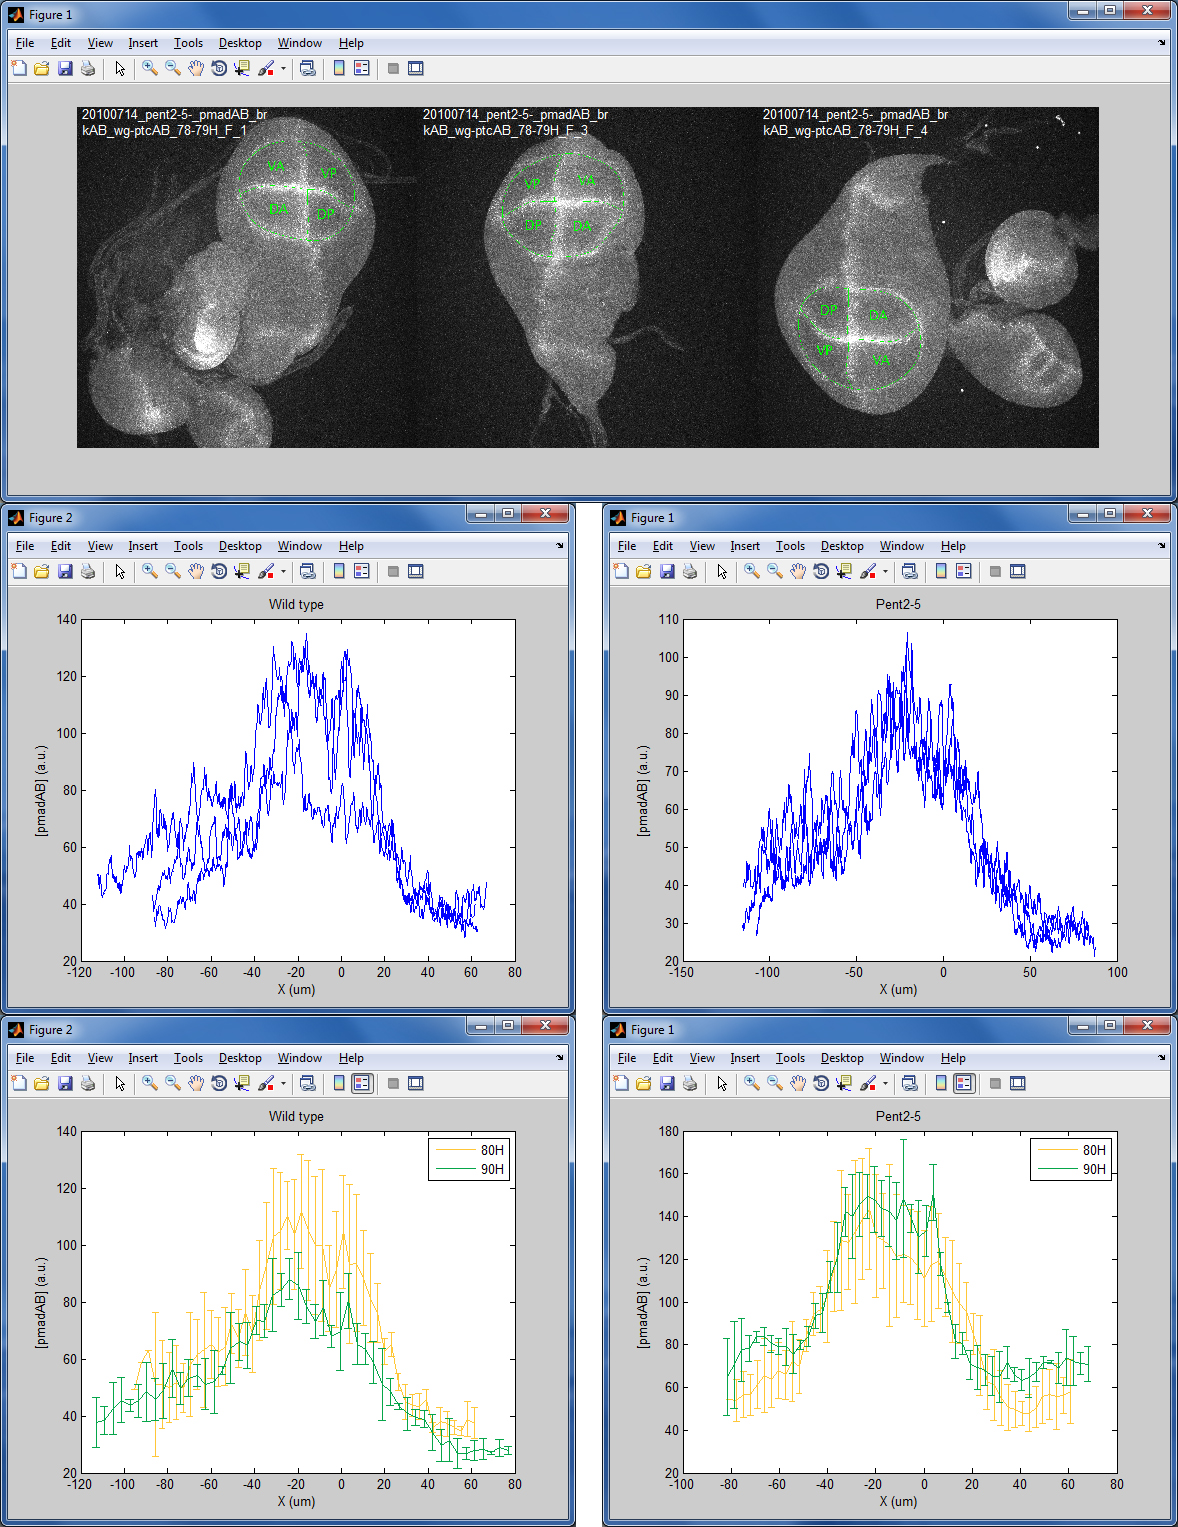
\includegraphics[scale=0.35]{images/matlab_expression_1D.jpg}
\caption{\textbf{Output of the \wingj \matlab script \textit{benchmark\_expression\_profiles.m}.} The top window shows the \textit{pent$^{2-5}$} mutant, 80-hour-old wings included in the folder \textit{benchmarks} which we provide along with the \wingjMatlab. Individual Pmad expression profiles measured along the D/V compartment boundary are reported for (left) wild type and (right) \textit{pent$^{2-5}$} mutant 80-hour-old wings. Finally, integrated expression profiles are computed (mean and standard deviation) and reported for both (left) wild type and (right) \textit{pent$^{2-5}$} mutant and for 80-hour- (yellow) and 90-hour-old (green) wings.}
\label{fig:matlab_expression_1D}
\end{figure}

The last line of the window displayed in \figureref{fig:matlab_expression_1D} shows the integrated expression profiles obtained for both wild type (left) and \textit{pent$^{2-5}$} mutant (right) and for 80-hour- (yellow) and 90-hour-old (green) wings. The integrated profiles show the mean and the standard deviation computed from the individual expression profiles (the number of points used to define the mean expression profile can be changed on the top part of \textit{benchmark\_expression\_profiles.m}).\\

\textbf{Tip:} Additional examples are available in \emph{examples/main\_expression\_profiles.m}. This file only provides descriptions and is not meant to be run.

% ===============================================================================
\section{Expression maps}
\wingj can be used to export individual expression maps, a representation we developed to quantify expression in 2D inside the space of the inferred structure model (\sectionref{sec:expression_maps}). The structure model, which is defined by its contour and the A/P and D/V compartment boundaries, provides a coordinate system that is used to build a parametric grid. The nodes of the grid give the locations where expression is sampled. The parametric grid looks different depending on the choice of the equator, which can be set along the A/P or D/V boundary. Example of individual \textit{circular expression maps} are shown in the top part of \figureref{fig:matlab_expression_2D}.\\

\begin{figure}[!h]
\centering
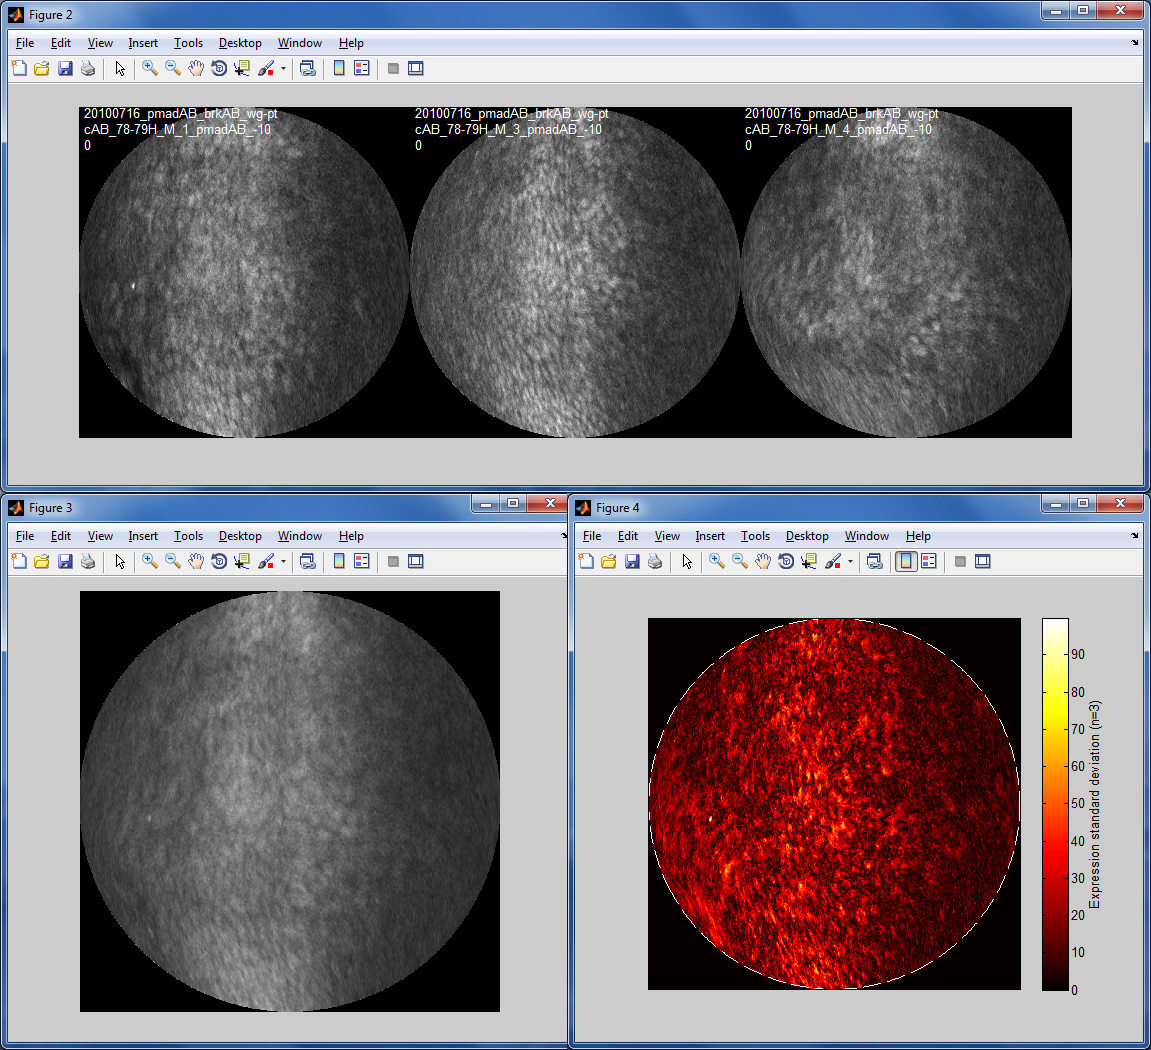
\includegraphics[scale=0.35]{images/matlab_expression_2D.jpg}
\caption{\textbf{Output of the \wingj \matlab script\textit{benchmark\_expression\_maps.m}.} The top window shows the individual \textit{circular expression maps} generated for wild type, 80-hour-old wings. Circular expression maps are computed from a structure model identified using \wingj (\sectionref{chap:structure}) and the mean projection of a stack of confocal fluorescence images (\sectionref{chap:expression}). The figure on the bottom corner is computed as the mean of the three individual expression maps. Moreover, the standard deviation (or distance) of expression levels is computed and reported in the bottom-right corner.}
\label{fig:matlab_expression_2D}
\end{figure}

We provide \matlab scripts to combine individual circular expression maps together in order to compute mean and standard deviation circular expression maps, for instance. \figureref{fig:matlab_expression_2D} (left) shows the mean circular expression map obtained by averaging the three maps shown in the top part of the same figure. The mean expression map provides a more reliable representation than an individual map and should always be considered for reliable analyses. Furthermore, circular expression maps allow to compare expression independently of the shape of the structure models considered. Therefore, they can be used to compare the difference in expression levels for wild type and mutant experiments, and for systems such as the \droso wing or embryo imaged at different time points (e.g. 80-hour- and 90-hour-old wings). In the same way that computing the mean expression map, \figureref{fig:matlab_expression_2D} (bottom-right) reports the distance (standard deviation) in term of expression levels measured between the three circular expression maps displayed on the top of this figure. This information can be used to study the conservation of expression in multiple wings at different locations inside the wing pouch or embryo, for instance.\\

\textbf{Important:} The circular representation of the expression maps has been developed as an intermediate description for averaging individual maps. The integration of individual expression maps is now performed in \wingj as part of the process to generate structure and expression aggregated models (\sectionref{sec:community_expression_maps}). However, this \matlab package becomes handy for generating custom circular expression maps such as those shown in \figureref{fig:wingj_expression_maps_circular_demo}. Note that \wingj provides the required tool to wrap any circular maps on top of any structure models inferred (\sectionref{sec:expression_reversed_maps}).\\

\textbf{Tip:} Additional examples are available in \emph{examples/main\_expression\_maps.m}. This file only provides descriptions and is not meant to be run.

% ===============================================================================
\section{3D cell nuclei detection}\label{sec:matlab_nuclei_detection}
From the structure model of the wing pouch or embryo structure inferred in \sectionref{chap:structure}, a 3D volume is generated within which the cell nuclei will be counted. This volume is obtained by extruding the contour of the 2D structure model in the $z$ dimension. Here, the nuclear staining we use is TO-PRO \autocite{schaffter2013}.\\

First, each slice from the TO-PRO image stack is pre-processed to remove noise and make the nuclei more visible. This is performed by applying successively different filters. Their respective output is shown in \figureref{fig:matlab_nuclei_detection_method}. Then, the 3D watershed algorithm implemented in \matlab is applied to segment the pre-processed images and reconstruct the nuclei in 3D before returning their number \autocite{meyer1994watershed}.\\

\begin{figure}[!h]
\centering
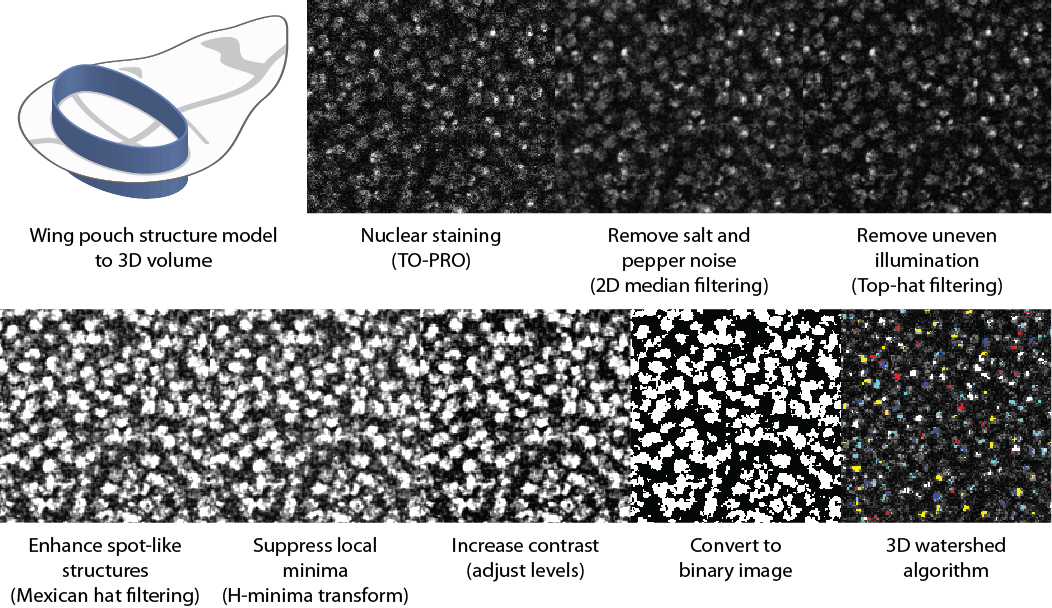
\includegraphics[scale=0.40]{images/matlab_nuclei_detection_method.jpg}
\caption{\textbf{Illustration of the 3D cell nuclei detection method available in the \wingjMatlab.} The structure model generated using \wingj (\sectionref{chap:structure}) is extruded to define a 3D volume within which cell nuclei will be identified from TO-PRO (a nuclear dye) confocal images \autocite{schaffter2013}. Each image slice is pre-processed before apply the 3D watershed algorithm implemented in \matlab to segment the images and reconstruct the 3D cell nuclei.}
\label{fig:matlab_nuclei_detection_method}
\end{figure}

It is important to mention that there are no methods that allow to identify every single nuclei from a stack of fluorescence confocal images (this is at least true for the nuclear dye we use). This comes mainly from the diffuse fluorescence that often makes it very difficult to distinct two close cell nuclei, even for human eyes. Thus, the method we propose only provides \textit{estimates} of the number of nuclei. However, these estimates already enable comparative analyzes, for instance by quantifying the relative difference in term of number of nuclei in batches of wings imaged at different time points. One can also quantify the effect of a mutation (e.g. \textit{pent$^{2-5}$}) on the number of nuclei in the \droso wing pouch compared to wild type experiments. A concrete example is given in \figureref{fig:matlab_nuclei_detection_num_nuclei} where the number of nuclei in the wing pouch is reported for wild type and \textit{pent$^{2-5}$} mutant wings and for different time points \autocite{schaffter2013}.\\

\begin{figure}[!h]
\centering
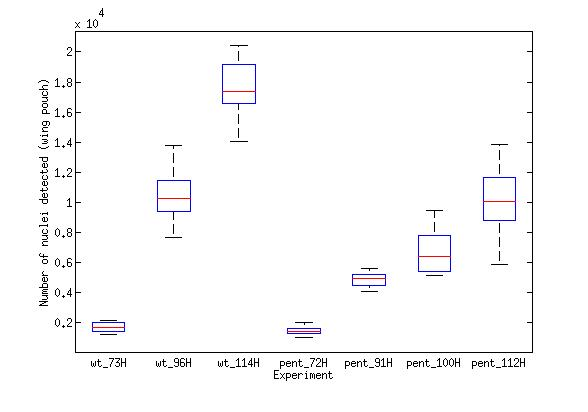
\includegraphics[scale=0.60]{images/matlab_nuclei_detection_num_nuclei.jpg}
\caption{\textbf{Number of nuclei identified in wild type and \textit{pent$^{2-5}$} mutant wings for different time points using the \wingj \matlab toolbox.} Nuclei detection is constrained to the space of the structure model previous identified using \wingj. This figure has been automatically generated using the tools of the \wingjMatlab.}
\label{fig:matlab_nuclei_detection_num_nuclei}
\end{figure}

The parameters of the nuclei detection method have been set to achieve accurate nuclei detection in our stacks of TO-PRO images. To evaluate the performance of our method, we have first defined a small volume as a subspace of an entire 3D image stack. Then, we manually counted the number of cell nuclei before setting the parameters of the nuclei detection methods so that its output is as close as possible to the result of the manual detection (ground truth). For accurate results, we strongly recommend that you perform a similar calibration for your images. The parameters to modify are in the method \textit{preProcess} of the \matlab script \textit{NucleiDetector}.\\

Run the \matlab script \textit{benchmark\_nuclei\_detection.m} to run the \wingj nuclei detection method on the three wings included in the folder \textit{benchmarks/20091222\_wg-ptcAB\_pentGFP\_TOPRO\_95,5-96,5H} (you may have to download the TO-PRO benchmark as a separate archive from \wingjShortUrl). At the end of the execution, a boxplot appears to report the number of nuclei found. More experiments (e.g. wings or embryos) are of course required to obtained meaningful statistics.\\

The script \textit{benchmark\_nuclei\_detection.m} contains the following instruction:\\

% \begin{codebox}
\footnotesize\texttt{\% Runs the nuclei detection of the wings included in \textit{wt\_TOPRO\_pentGFP\_95H}\\
wt\_TOPRO\_pentGFP\_95H.get(:).detectNuclei('TOPRO',[],true);}\normalsize\\
% \end{codebox}

This instruction runs the nuclei detection on every wings listed in the \textit{ExperimentList} object \textit{wt\_TOPRO\_pentGFP\_95H}, which here includes three wings. If the method \textit{detectNuclei} is run without the second (slice indexes to take into account, \textit{[]} means using all of them) and third argument (if true, saves the individual processed images and an AVI video made out of them), the nuclei detection saves only the number of nuclei detected to a file in text format. This file is saved in the folder \textit{WingJ/Matlab/NucleiDetector/} included in each experiment folder (\sectionref{sec:experiment_directory}). If the third argument is \textit{true}, the selected slices from the TO-PRO stack are exported in TIFF format where the sections of the nuclei identified are shown in different colors. Moreover, a video made out of these images is automatically exported in AVI format (the FPS of the video can be changed in the \wingj \matlab \emph{Settings} file). \figureref{fig:watershed} shows one image from the video where the detected cell nuclei are labelled with different colors. Once again and thanks to the structure model identified using \wingj, the nuclei detection can be constrained to a subspace of the entire image stacks (here the wing pouch organ system).\\

\begin{figure}[!h]
\centering
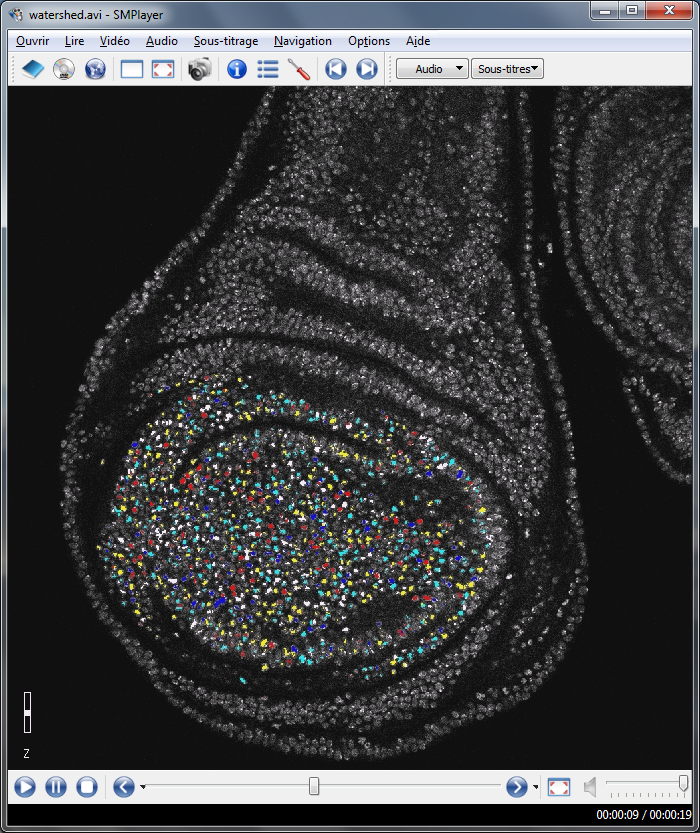
\includegraphics[scale=0.40]{images/watershed.jpg}
\caption{\textbf{Illustration of the output of the 3D cell nuclei detection method.} The nuclei detection method we propose in the \wingjMatlab exports videos in AVI format where the nuclei identified inside the space of the structure model (here the wing pouch organ system) are labelled with different colors. The video and the individual images that were used to make it are exported to the folder \textit{WingJ/Matlab/NucleiDetector/} of each experiment folder.}
\label{fig:watershed}
\end{figure}

\textbf{Tip:} Additional examples are available in \emph{examples/main\_nuclei\_detection.m}. This file only provides descriptions and is not meant to be run.